
\usetikzlibrary{calc}

\def\placeCoords{%
\coordinate (e0) at (0,0,0);
\coordinate (e1) at (1,0,0);
\coordinate (e2) at (0,0,-1);
\coordinate (e3) at (-1,0,0);
\coordinate (e4) at (0,0,1) ;
\coordinate (e5) at (0,1,0) ;
\coordinate (e6) at (0,-1,0);
\coordinate (e7) at (1,0,-1);
\coordinate (e8) at (-1,0,-1);
\coordinate (e9) at (-1,0,1);
\coordinate (e10) at (1,0,1) ;
\coordinate (e11) at (1,1,0) ;
\coordinate (e12) at (-1,1,0);
\coordinate (e13) at (-1,-1,0);
\coordinate (e14) at (1,-1,0);
\coordinate (e15) at (0,1,-1);
\coordinate (e16) at (0,1,1) ;
\coordinate (e17) at (0,-1,1);
\coordinate (e18) at (0,-1,-1);
\coordinate (e19) at (1,1,-1);
\coordinate (e20) at (-1,1,-1);
\coordinate (e21) at (-1,1,1);
\coordinate (e22) at (1,1,1);
\coordinate (e23) at (1,-1,-1);
\coordinate (e24) at (-1,-1,-1);
\coordinate (e25) at (-1,-1,1);
\coordinate (e26) at (1,-1,1);
}

\def\drawBox{%
\draw[dashed] (-1,-1,0) rectangle + (2,2,0);
\draw[dashed] (-1,-1,-1) rectangle + (2,2,0);
\draw[dashed] (-1,-1,1) rectangle + (2,2,0);
\draw[dashed] (-1,-1,-1) -- (-1,-1,1);
\draw[dashed] (1,1,-1) -- (1,1,1);
\draw[dashed] (-1,1,-1) -- (-1,1,1);
\draw[dashed] (1,-1,-1) -- (1,-1,1);
\draw[dashed] (-1,0,1) -- (1,0,1) -- (1,0,-1) -- (-1,0,-1) -- (-1,0,1);
\draw[dashed] (0,-1,1) -- (0,1,1) -- (0,1,-1) -- (0,-1,-1) -- (0,-1,1);
}
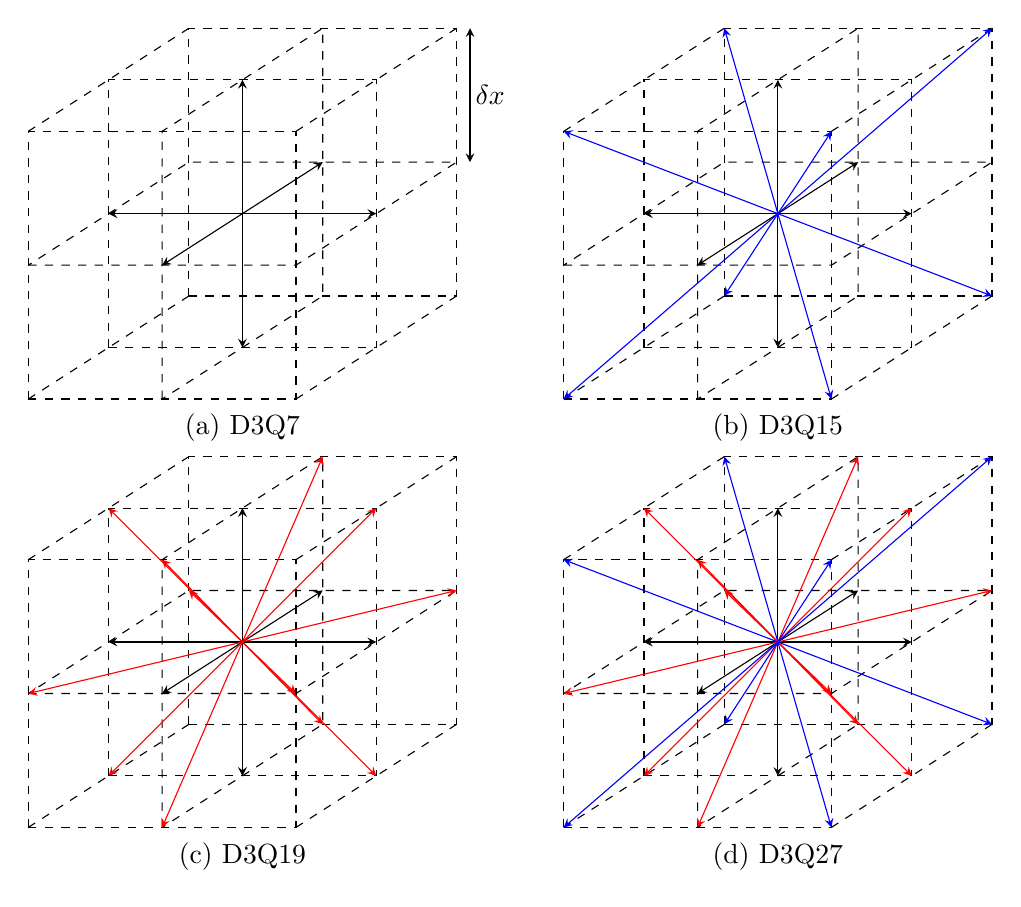
\begin{tikzpicture}[x={(1cm,0cm)}, y={(0cm,1cm)}, z={(-6mm, -3.85mm)}, scale=1.7]

%styledesnœuds
\tikzstyle{textLine}=[rectangle, text=black,scale=1]
\tikzstyle{textw}=[rectangle, text=black]


% styles
\tikzstyle{pointEi}=[circle, fill, scale=0.2]
\tikzstyle{pointEiQ19}=[circle, fill, scale=0.2, color=red]
\tikzstyle{pointEiQ15}=[circle, fill, scale=0.2, color=blue]

\tikzstyle{vector}=[-{stealth[scale=0.5]},thin,rounded corners=4pt]
\tikzstyle{vectorQ19}=[-{stealth[scale=0.5]},thin, rounded corners=4pt, color=red]
\tikzstyle{vectorQ15}=[-{stealth[scale=0.5]},thin, rounded corners=4pt, color=blue]



\begin{scope}[shift={(0,0,0)}]
\node[textLine] at (0,-1.6) {(a) D3Q7};
\drawBox
\placeCoords

\draw[vector] (e0) -- (e1);
\draw[vector] (e0) -- (e2);
\draw[vector] (e0) -- (e3);
\draw[vector] (e0) -- (e4);
\draw[vector] (e0) -- (e5);
\draw[vector] (e0) -- (e6);

\draw[stealth-stealth] ($(e7)+(0.1,0,0)$) -- ($(e19)+(0.1,0,0)$);
\node[textLine] at ($($(e7)+(0.25,0,0)$)!0.5!($(e19)+(0.25,0,0)$)$) {$\delta x$};
\end{scope}


\begin{scope}[shift={(4,0,0)}]
\node[textLine] at (0,-1.6) {(b) D3Q15};
\drawBox
\placeCoords

\draw[vector] (e0) -- (e1);
\draw[vector] (e0) -- (e2);
\draw[vector] (e0) -- (e3);
\draw[vector] (e0) -- (e4);
\draw[vector] (e0) -- (e5);
\draw[vector] (e0) -- (e6);
\draw[vectorQ15] (e0) -- (e19);
\draw[vectorQ15] (e0) -- (e20);
\draw[vectorQ15] (e0) -- (e21);
\draw[vectorQ15] (e0) -- (e22);
\draw[vectorQ15] (e0) -- (e23);
\draw[vectorQ15] (e0) -- (e24);
\draw[vectorQ15] (e0) -- (e25);
\draw[vectorQ15] (e0) -- (e26);
\end{scope}

\begin{scope}[shift={(0,-3.2,0)}]
\node[textLine] at (0,-1.6) {(c) D3Q19};
\drawBox
\placeCoords

\draw[vector] (e0) -- (e1);
\draw[vector] (e0) -- (e2);
\draw[vector] (e0) -- (e3);
\draw[vector] (e0) -- (e4);
\draw[vector] (e0) -- (e5);
\draw[vector] (e0) -- (e6);
\draw[vectorQ19] (e0) -- (e7);
\draw[vectorQ19] (e0) -- (e8);
\draw[vectorQ19] (e0) -- (e9);
\draw[vectorQ19] (e0) -- (e10);
\draw[vectorQ19] (e0) -- (e11);
\draw[vectorQ19] (e0) -- (e12);
\draw[vectorQ19] (e0) -- (e13);
\draw[vectorQ19] (e0) -- (e14);
\draw[vectorQ19] (e0) -- (e15);
\draw[vectorQ19] (e0) -- (e16);
\draw[vectorQ19] (e0) -- (e17);
\draw[vectorQ19] (e0) -- (e18);
\end{scope}

\begin{scope}[shift={(4,-3.2,0)}]
\node[textLine] at (0,-1.6) {(d) D3Q27};
\drawBox
\placeCoords

\draw[vector] (e0) -- (e1);
\draw[vector] (e0) -- (e2);
\draw[vector] (e0) -- (e3);
\draw[vector] (e0) -- (e4);
\draw[vector] (e0) -- (e5);
\draw[vector] (e0) -- (e6);
\draw[vectorQ19] (e0) -- (e7);
\draw[vectorQ19] (e0) -- (e8);
\draw[vectorQ19] (e0) -- (e9);
\draw[vectorQ19] (e0) -- (e10);
\draw[vectorQ19] (e0) -- (e11);
\draw[vectorQ19] (e0) -- (e12);
\draw[vectorQ19] (e0) -- (e13);
\draw[vectorQ19] (e0) -- (e14);
\draw[vectorQ19] (e0) -- (e15);
\draw[vectorQ19] (e0) -- (e16);
\draw[vectorQ19] (e0) -- (e17);
\draw[vectorQ19] (e0) -- (e18);
\draw[vectorQ15] (e0) -- (e19);
\draw[vectorQ15] (e0) -- (e20);
\draw[vectorQ15] (e0) -- (e21);
\draw[vectorQ15] (e0) -- (e22);
\draw[vectorQ15] (e0) -- (e23);
\draw[vectorQ15] (e0) -- (e24);
\draw[vectorQ15] (e0) -- (e25);
\draw[vectorQ15] (e0) -- (e26);
\end{scope}





\end{tikzpicture}
